In this chapter, we will provide a general project schedule. More refined schedule will be provided during project development, in order to reflect eventual changes. Even if this project is made only for didactic purpose we will provided a hypothetical schedule of the development phase of the project, that we will not deal with.  This is to mimic how a real project should work.
In order to maintain readability, we split the schedule into five parts: one for the RASD, one for the DD, one for the ITPS and PPD and two for the development.

\begin{center}
  \makebox[\textwidth]{
    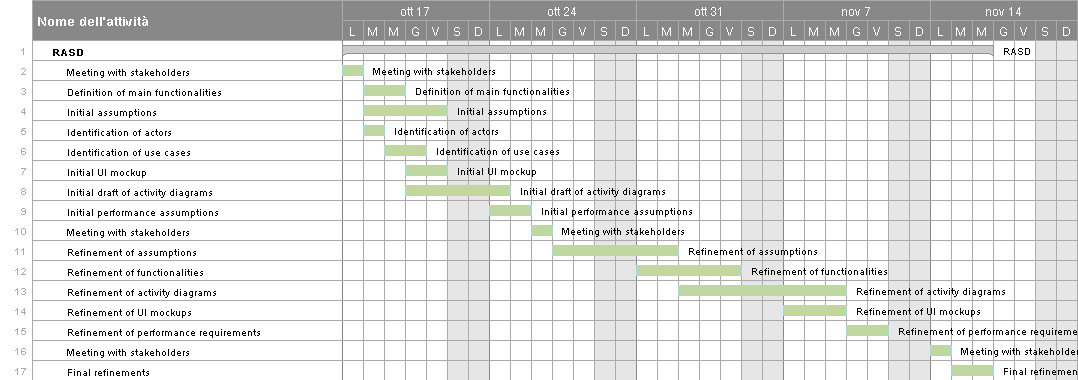
\includegraphics[width=\paperwidth]{schedule/RASD.png}
	}
\end{center}

\begin{center}
  \makebox[\textwidth]{
    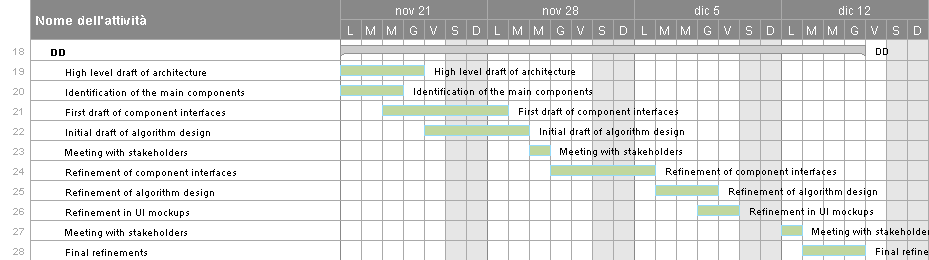
\includegraphics[width=\paperwidth]{schedule/DD.png}
	}
\end{center}

\begin{center}
  \makebox[\textwidth]{
    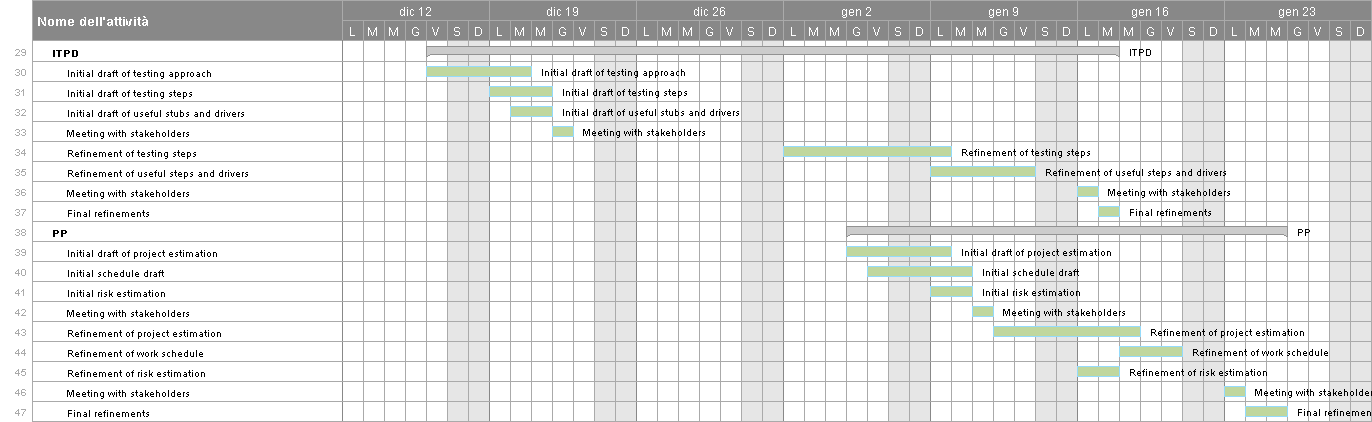
\includegraphics[width=\paperwidth]{schedule/ITDP_PP.png}
	}
\end{center}

\begin{center}
  \makebox[\textwidth]{
    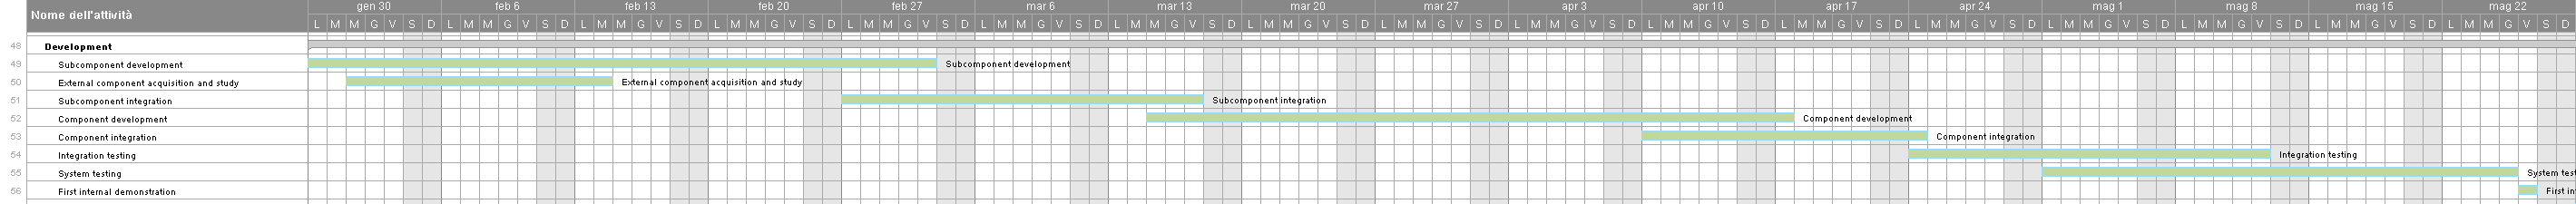
\includegraphics[width=\paperwidth]{schedule/Develop1.png}
	}
\end{center}

\begin{center}
  \makebox[\textwidth]{
    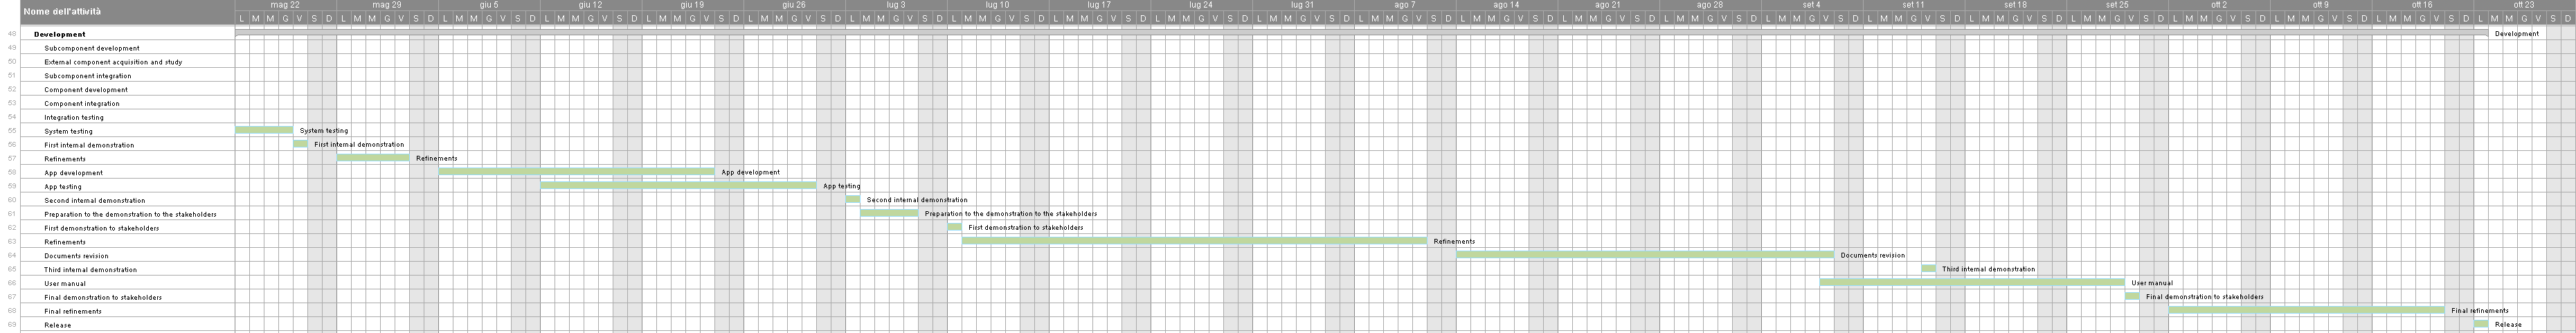
\includegraphics[width=\paperwidth]{schedule/Develop2.png}
	}
\end{center}